% Unofficial UChicago CS Poster Template
% v1.1.0 released September 8, 2022
% https://github.com/k4rtik/uchicago-poster
% a fork of https://github.com/anishathalye/gemini

\documentclass[final]{beamer}

% ====================
% Packages
% ====================

\usepackage[T1]{fontenc}
\usepackage{lmodern}
\usepackage[size=custom,width=120,height=72,scale=1.0]{beamerposter}
\usetheme{gemini}
\usecolortheme{jhu}
\usepackage{graphicx}
\usepackage{booktabs}
\usepackage{doi}
\usepackage[numbers]{natbib}
\usepackage[patch=none]{microtype}
\usepackage{tikz}
\usepackage{pgfplots}
\pgfplotsset{compat=1.18}
\usepackage{anyfontsize}
\usepackage{subcaption}
\usepackage{multirow}
\usepackage{booktabs}

\pdfstringdefDisableCommands{%
\def\translate#1{#1}%
}

% ====================
% Lengths
% ====================

% If you have N columns, choose \sepwidth and \colwidth such that
% (N+1)*\sepwidth + N*\colwidth = \paperwidth
\newlength{\sepwidth}
\newlength{\colwidth}
\setlength{\sepwidth}{0.025\paperwidth}
\setlength{\colwidth}{0.3\paperwidth}

\newcommand{\separatorcolumn}{\begin{column}{\sepwidth}\end{column}}

% ====================
% Title
% ====================

\title{Deep Semantic Statistics Matching Denoising Network}

\author{Kangfu Mei \and Vishal M. Patel \and Rui Huang}

\institute[shortinst]{Johns Hopkins University \samelineand The Chinese University of Hong Kong, Shenzhen}

% ====================
% Footer (optional)
% ====================

% \footercontent{
%   \href{https://www.example.com}{https://www.example.com} \hfill
%   ABC Conference 2025, New York --- XYZ-1234 \hfill
%   \href{mailto:alyssa.p.hacker@example.com}{alyssa.p.hacker@example.com}}
% (can be left out to remove footer)

% ====================
% Logo (optional)
% ====================

% use this to include logos on the left and/or right side of the header:
% \logoright{\includegraphics[height=7cm]{logo1.pdf}}
% \logoleft{\includegraphics[height=7cm]{logo2.pdf}}

% ====================
% Body
% ====================

\begin{document}
\addtobeamertemplate{headline}{}
{
    \begin{tikzpicture}[remember picture,overlay]
      \node [anchor=north west, inner sep=3cm] at ([xshift=0.0cm,yshift=1.0cm]current page.north west)
      {
\includegraphics[height=5.0cm]{jhu-logos/university.shield.white.eps}
\includegraphics[height=5.0cm]{cuhk.png}}; % also try shield-white.eps
      \node [anchor=north east, inner sep=3cm] at ([xshift=0.0cm,yshift=1.5cm]current page.north east)
      {
\includegraphics[height=5.0cm]{ECCV-logo.png}};
    \end{tikzpicture}
}

\begin{frame}[t]
\begin{columns}[t]
\separatorcolumn

\begin{column}{\colwidth}

  \begin{block}{TL;DR}
  \textbf{A new framework for generalizing image restoration networks on high-level vision tasks.}
  \begin{figure}
      \centering
      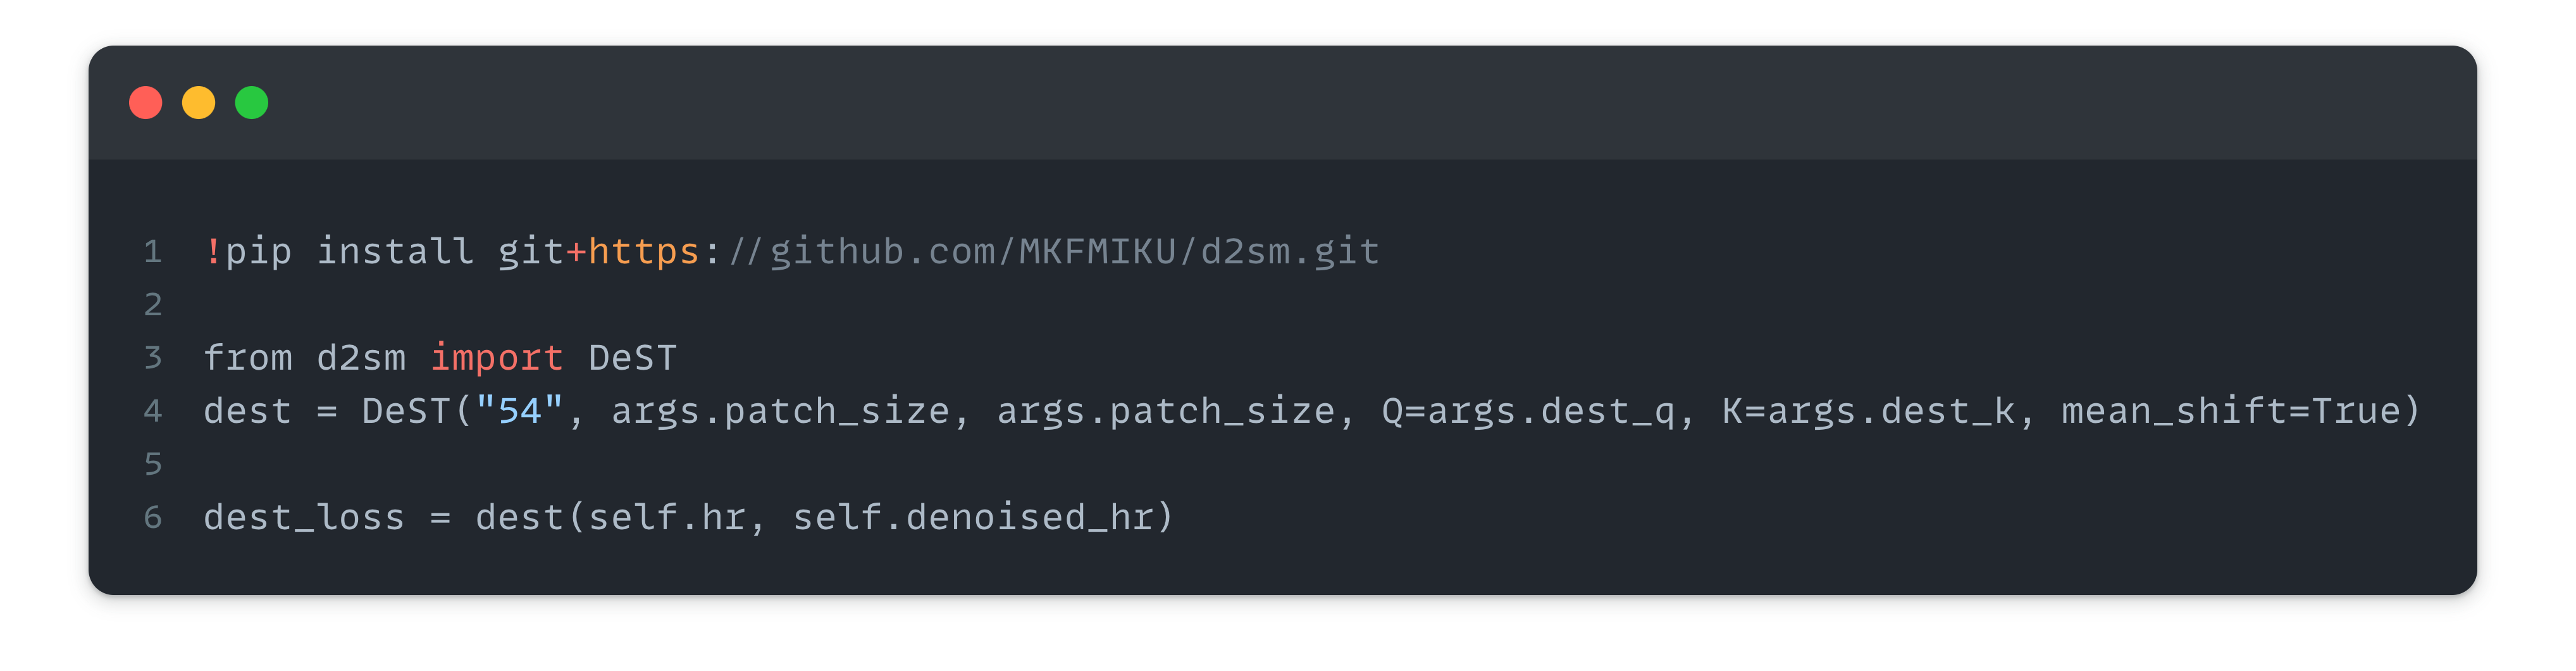
\includegraphics[width=\linewidth]{contents/code.png}
  \end{figure}

  \end{block}

  \begin{block}{Problem Settings}

  \begin{figure}
  \begin{subfigure}[c]{.22\linewidth}
    \captionsetup{justification=centering, labelformat=empty, font=small}
    \includegraphics[width=1\linewidth]{contents/feature-space/l1.pdf}
    \caption{w. $\mathcal{L}_1$}
  \end{subfigure}
  \hfill
  \begin{subfigure}[c]{.22\linewidth}
    \captionsetup{justification=centering, labelformat=empty, font=small}
    \includegraphics[width=1\linewidth]{contents/feature-space/vgg.pdf}
    \caption{w. $\mathcal{L}_{Perceptual}$}
  \end{subfigure}
  \hfill
  \begin{subfigure}[c]{.22\linewidth}
    \captionsetup{justification=centering, labelformat=empty, font=small}
    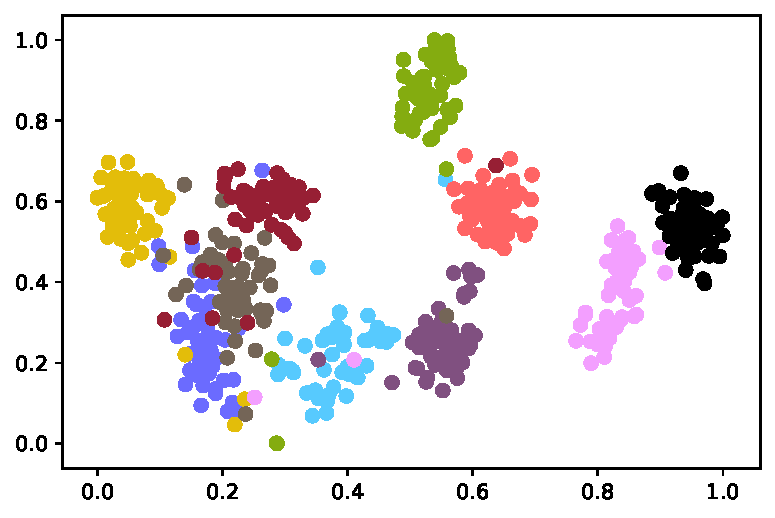
\includegraphics[width=1\linewidth]{contents/feature-space/dst.pdf}
    \caption{Ours}
  \end{subfigure}
  \hfill
  \begin{subfigure}[c]{.285\linewidth}
    \captionsetup{justification=centering, labelformat=empty, font=small}
    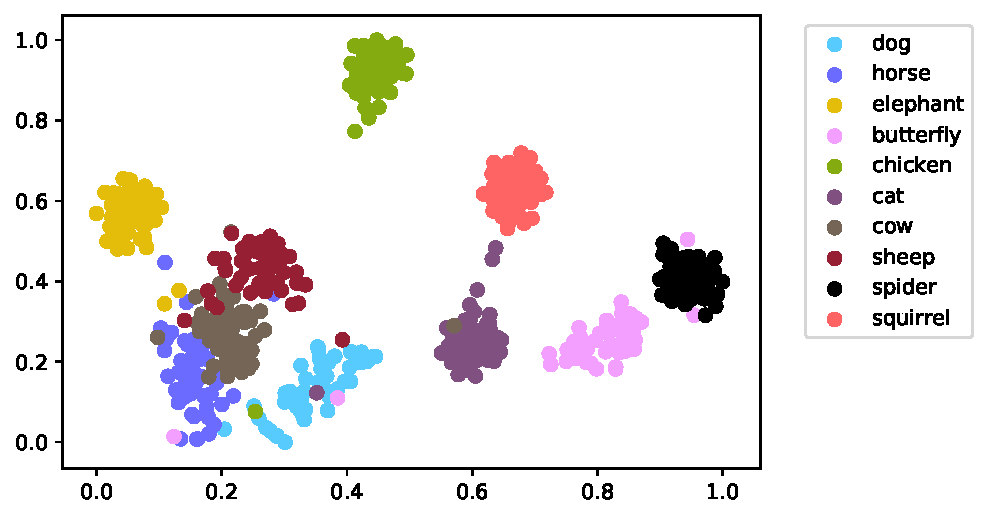
\includegraphics[width=1\linewidth]{contents/feature-space/gt.pdf}
    \caption{Clear Images}
  \end{subfigure}  
  \vspace{-.2in}
  \caption{\textbf{t-SNE of denoised Images in the Semantic Feature Space.} Ours preserves most semantics like GT.}
\end{figure}


  \end{block}

  \begin{alertblock}{Contributions}

  \end{alertblock}

\end{column}

\separatorcolumn

\begin{column}{\colwidth}

  \begin{block}{Method}
  \begin{figure}
      \centering
      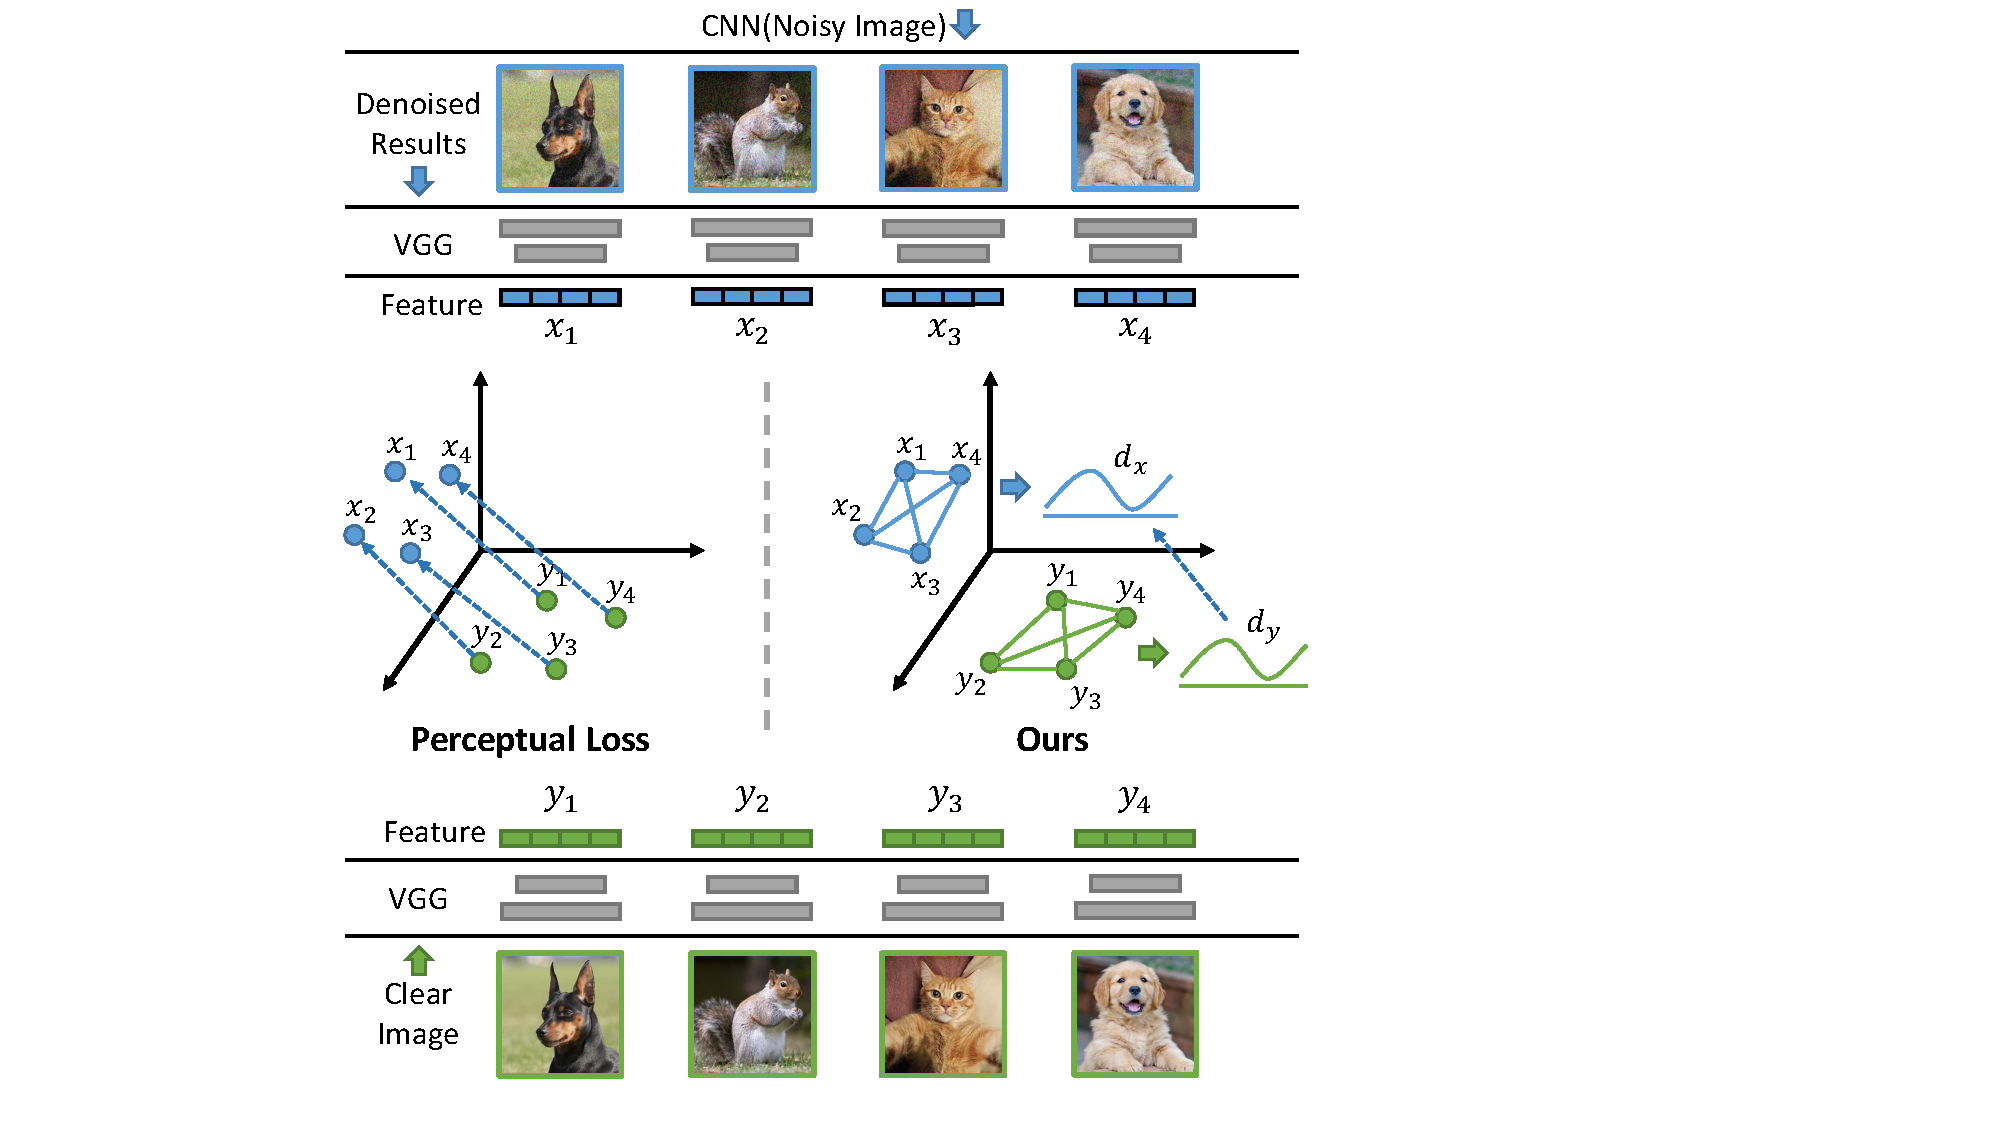
\includegraphics[width=.8\linewidth]{contents/teaser-2.pdf}
      \caption{\textbf{Perceptual loss vs. Ours.}}
  \end{figure}

  \end{block}

  \begin{block}{Experiment Details}


  \end{block}

\end{column}

\separatorcolumn

\begin{column}{\colwidth}

  \begin{exampleblock}{Results}

    \heading{Cityscape Denoising and Segmentation}
    \begin{table}[htbp]
	\centering
	\caption{\textbf{Quantitative performance comparison on the cityscape denoising and segmentation.}}
	\resizebox{\linewidth}{!}{
		\begin{tabular}{llccccccccc}
			\toprule
			& & \multicolumn{3}{c}{Noise-Level $\sigma$=25} & \multicolumn{3}{c}{Noise-Level $\sigma$=35} & \multicolumn{3}{c}{Noise-Level $\sigma$=50} \\
			\cmidrule(r){3-5} \cmidrule(r){6-8} \cmidrule(r){9-11} Method (Backbone) & Objective                                                   & PSNR $\uparrow$         & SSIM $\uparrow$        & MIoU (\%) $\uparrow$   & PSNR $\uparrow$         & SSIM $\uparrow$        & MIoU (\%) $\uparrow$   & PSNR $\uparrow$         & SSIM $\uparrow$        & MIoU (\%) $\uparrow$   \\
			\midrule[1pt]
			\multirow{6}{*}{FFDNet~\cite{zhang_ffdnet_2018}}                         & $\mathcal{L}_1$                                             & 35.033$^{(6)}$          & 0.925$^{(6)}$          & 0.605$^{(8)}$          & 34.074$^{(6)}$          & 0.912$^{(6)}$          & 0.537$^{(8)}$          & 32.845$^{(6)}$          & 0.895$^{(6)}$          & 0.451$^{(7)}$          \\
			                                                                         & + $\mathcal{L}_{SSIM}$               & 35.567$^{(3)}$          & 0.935$^{(2)}$          & 0.642$^{(2)}$          & 34.469$^{(4)}$          & 0.922$^{(2)}$          & 0.584$^{(2)}$          & 33.180$^{(3)}$          & 0.906$^{(2)}$          & 0.450$^{(8)}$          \\
			                                                                         & + $\mathcal{L}_{Perceptual}$ & 34.319$^{(7)}$          & 0.912$^{(7)}$          & 0.629$^{(4)}$          & 33.486$^{(7)}$          & 0.899$^{(7)}$          & 0.582$^{(4)}$          & 32.383$^{(7)}$          & 0.881$^{(7)}$          & 0.509$^{(2)}$          \\
			                                                                         & + $\mathcal{L}_{LPIPS}$      & 35.551$^{(4)}$          & 0.929$^{(4)}$          & 0.613$^{(6)}$          & 34.463$^{(5)}$          & 0.916$^{(4)}$          & 0.541$^{(7)}$          & 33.138$^{(5)}$          & 0.899$^{(4)}$          & 0.452$^{(6)}$          \\
			                                                                         & + $\mathcal{L}_{Contextual}$ & 25.115$^{(8)}$          & 0.762$^{(8)}$          & 0.628$^{(5)}$          & 24.938$^{(8)}$          & 0.758$^{(8)}$          & 0.583$^{(3)}$          & 24.775$^{(8)}$          & 0.753$^{(8)}$          & 0.509$^{(2)}$          \\
			                                                                         & + $\mathcal{L}_{CrossEntropy}$   & 35.913$^{(2)}$          & 0.932$^{(3)}$          & 0.630$^{(3)}$          & 34.800$^{(2)}$          & 0.919$^{(3)}$          & 0.565$^{(5)}$          & 33.477$^{(2)}$          & 0.903$^{(3)}$          & 0.491$^{(4)}$          \\
			\hline\multirow{2}{*}{D2SM (Ours)}                                       & w/o. Internal                                               & 35.543$^{(5)}$          & 0.929$^{(4)}$          & 0.612$^{(7)}$          & 34.475$^{(3)}$          & 0.916$^{(4)}$          & 0.546$^{(6)}$          & 33.167$^{(4)}$          & 0.899$^{(4)}$          & 0.463$^{(5)}$          \\
			                                                                         & w/. Internal                                                & \textbf{36.454$^{(1)}$} & \textbf{0.936$^{(1)}$} & \textbf{0.644$^{(1)}$} & \textbf{35.206$^{(1)}$} & \textbf{0.923$^{(1)}$} & \textbf{0.587$^{(1)}$} & \textbf{33.807$^{(1)}$} & \textbf{0.907$^{(1)}$} & \textbf{0.520$^{(1)}$} \\
			  
			\hline
			\hline
			\multirow{3}{*}{CBDNet~\cite{guo_toward_2019}}                           & -                                                           & 36.152$^{(3)}$          & 0.936$^{(2)}$          & 0.655$^{(3)}$          & 34.964$^{(3)}$          & 0.923$^{(3)}$          & 0.599$^{(3)}$          & 33.613$^{(3)}$          & 0.907$^{(3)}$          & 0.539$^{(3)}$          \\
			                                                                         & w/o. Internal                                               & 36.254$^{(2)}$          & 0.935$^{(3)}$          & 0.679$^{(2)}$          & 35.158$^{(2)}$          & 0.925$^{(2)}$          & 0.631$^{(2)}$          & 33.904$^{(2)}$          & 0.911$^{(2)}$          & 0.550$^{(2)}$          \\
			                                                                         & w/. Internal                                                & \textbf{36.899$^{(1)}$} & \textbf{0.941$^{(1)}$} & \textbf{0.691$^{(1)}$} & \textbf{35.596$^{(1)}$} & \textbf{0.929$^{(1)}$} & \textbf{0.652$^{(1)}$} & \textbf{34.172$^{(1)}$} & \textbf{0.914$^{(1)}$} & \textbf{0.600$^{(1)}$} \\
			\hline
			\hline
			\multirow{3}{*}{SADNet~\cite{chang_spatial-adaptive_2020}}               & -                                                           & 36.310$^{(3)}$          & 0.936$^{(3)}$          & 0.674$^{(3)}$          & 35.081$^{(3)}$          & 0.924$^{(2)}$          & 0.637$^{(3)}$          & 33.730$^{(3)}$          & 0.908$^{(3)}$          & 0.581$^{(3)}$          \\
			                                                                         & w/o. Internal                                               & 36.822$^{(2)}$          & 0.940$^{(2)}$          & 0.691$^{(2)}$          & 35.247$^{(2)}$          & 0.924$^{(2)}$          & 0.655$^{(2)}$          & 34.133$^{(2)}$          & 0.912$^{(2)}$          & 0.600$^{(2)}$          \\
			                                                                         & w/. Internal                                                & \textbf{37.130$^{(1)}$} & \textbf{0.943$^{(1)}$} & \textbf{0.701$^{(1)}$} & \textbf{35.839$^{(1)}$} & \textbf{0.931$^{(1)}$} & \textbf{0.670$^{(1)}$} & \textbf{34.440$^{(1)}$} & \textbf{0.916$^{(1)}$} & \textbf{0.634$^{(1)}$} \\
			\bottomrule
		\end{tabular}}
\end{table}
    
\begin{figure}[htbp]
    \begin{subfigure}[t]{.195\linewidth}
      \captionsetup{justification=centering, labelformat=empty, font=scriptsize}
      \setlength{\fboxrule}{1pt}
      \setlength{\fboxsep}{0pt}
      \fcolorbox{blue}{white}{\includegraphics[width=0.45\linewidth]{figures/visualization/munster_000155_000019_25_highlight1/data.png}}
      \fcolorbox{red}{white}{\includegraphics[width=0.45\linewidth]{figures/visualization/munster_000155_000019_25_highlight2/data.png}}
      \includegraphics[width=1.\linewidth]{figures/visualization/mark/data.png}
      \caption{Noisy Image \\ Acc: 23.66\%}
    \end{subfigure}%
    \hfill
    \begin{subfigure}[t]{.195\linewidth}
      \captionsetup{justification=centering, labelformat=empty, font=scriptsize}
      \setlength{\fboxrule}{1pt}
      \setlength{\fboxsep}{0pt}
      \fcolorbox{blue}{white}{\includegraphics[width=0.45\linewidth]{figures/visualization/munster_000155_000019_25_highlight1/l1.png}}
      \fcolorbox{red}{white}{\includegraphics[width=0.45\linewidth]{figures/visualization/munster_000155_000019_25_highlight2/l1.png}}
      \fcolorbox{green}{white}{\includegraphics[width=0.45\linewidth]{figures/visualization/munster_000155_000019_25_highlight3/seg_l1.png}}
      \fcolorbox{green}{white}{\includegraphics[width=0.45\linewidth]{figures/visualization/munster_000155_000019_25_highlight4/seg_l1.png}}
      \caption{$\mathcal{L}_1$ \\ Acc: 42.59\%}
    \end{subfigure}%
    \hfill
    \begin{subfigure}[t]{.195\linewidth}
      \captionsetup{justification=centering, labelformat=empty, font=scriptsize}
      \setlength{\fboxrule}{1pt}
      \setlength{\fboxsep}{0pt}
      \fcolorbox{blue}{white}{\includegraphics[width=0.45\linewidth]{figures/visualization/munster_000155_000019_25_highlight1/ssim.png}}
      \fcolorbox{red}{white}{\includegraphics[width=0.45\linewidth]{figures/visualization/munster_000155_000019_25_highlight2/ssim.png}}
      \fcolorbox{green}{white}{\includegraphics[width=0.45\linewidth]{figures/visualization/munster_000155_000019_25_highlight3/seg_ssim.png}}
      \fcolorbox{green}{white}{\includegraphics[width=0.45\linewidth]{figures/visualization/munster_000155_000019_25_highlight4/seg_ssim.png}}
      \caption{$\mathcal{L}_{SSIM}$~\cite{wang_image_2004} \\ Acc: 44.84\%}
    \end{subfigure}%
    \hfill
    \begin{subfigure}[t]{.195\linewidth}
      \captionsetup{justification=centering, labelformat=empty, font=scriptsize}
      \setlength{\fboxrule}{1pt}
      \setlength{\fboxsep}{0pt}
      \fcolorbox{blue}{white}{\includegraphics[width=0.45\linewidth]{figures/visualization/munster_000155_000019_25_highlight1/vgg.png}}
      \fcolorbox{red}{white}{\includegraphics[width=0.45\linewidth]{figures/visualization/munster_000155_000019_25_highlight2/vgg.png}}
      \fcolorbox{green}{white}{\includegraphics[width=0.45\linewidth]{figures/visualization/munster_000155_000019_25_highlight3/seg_vgg.png}}
      \fcolorbox{green}{white}{\includegraphics[width=0.45\linewidth]{figures/visualization/munster_000155_000019_25_highlight4/seg_vgg.png}}
      \caption{$\mathcal{L}_{Perceptual}$~\cite{johnson_perceptual_2016} \\ Acc: 45.35\%}
    \end{subfigure}%
    \hfill
    \begin{subfigure}[t]{.195\linewidth}
      \captionsetup{justification=centering, labelformat=empty, font=scriptsize}
      \setlength{\fboxrule}{1pt}
      \setlength{\fboxsep}{0pt}
      \fcolorbox{blue}{white}{\includegraphics[width=0.45\linewidth]{figures/visualization/munster_000155_000019_25_highlight1/lpips.png}}
      \fcolorbox{red}{white}{\includegraphics[width=0.45\linewidth]{figures/visualization/munster_000155_000019_25_highlight2/lpips.png}}
      \fcolorbox{green}{white}{\includegraphics[width=0.45\linewidth]{figures/visualization/munster_000155_000019_25_highlight3/seg_lpips.png}}
      \fcolorbox{green}{white}{\includegraphics[width=0.45\linewidth]{figures/visualization/munster_000155_000019_25_highlight4/seg_lpips.png}}
      \caption{$\mathcal{L}_{LPIPS}$~\cite{zhang_unreasonable_2018} \\ Acc: 43.25\%}
    \end{subfigure}%
  
    \begin{subfigure}[t]{.195\linewidth}
      \captionsetup{justification=centering, labelformat=empty, font=scriptsize}
      \setlength{\fboxrule}{1pt}
      \setlength{\fboxsep}{0pt}
      \fcolorbox{blue}{white}{\includegraphics[width=0.45\linewidth]{figures/visualization/munster_000155_000019_25_highlight1/cx.png}}
      \fcolorbox{red}{white}{\includegraphics[width=0.45\linewidth]{figures/visualization/munster_000155_000019_25_highlight2/cx.png}}
      \fcolorbox{green}{white}{\includegraphics[width=0.45\linewidth]{figures/visualization/munster_000155_000019_25_highlight3/seg_cx.png}}
      \fcolorbox{green}{white}{\includegraphics[width=0.45\linewidth]{figures/visualization/munster_000155_000019_25_highlight4/seg_cx.png}}
      \caption{$\mathcal{L}_{Contextual}$~\cite{mechrez_contextual_2018} \\ Acc: 43.28\%}
    \end{subfigure}%
    \hfill
    \begin{subfigure}[t]{.195\linewidth}
      \captionsetup{justification=centering, labelformat=empty, font=scriptsize}
      \setlength{\fboxrule}{1pt}
      \setlength{\fboxsep}{0pt}
      \fcolorbox{blue}{white}{\includegraphics[width=0.45\linewidth]{figures/visualization/munster_000155_000019_25_highlight1/semantic-label.png}}
      \fcolorbox{red}{white}{\includegraphics[width=0.45\linewidth]{figures/visualization/munster_000155_000019_25_highlight2/semantic-label.png}}
      \fcolorbox{green}{white}{\includegraphics[width=0.45\linewidth]{figures/visualization/munster_000155_000019_25_highlight3/seg_semantic-label.png}}
      \fcolorbox{green}{white}{\includegraphics[width=0.45\linewidth]{figures/visualization/munster_000155_000019_25_highlight4/seg_semantic-label.png}}
      \caption{$\mathcal{L}_{CrossEntropy}$~\cite{liu_connecting_2020} \\ Acc: 44.09\%}
    \end{subfigure}%
    \hfill
    \begin{subfigure}[t]{.195\linewidth}
      \captionsetup{justification=centering, labelformat=empty, font=scriptsize}
      \setlength{\fboxrule}{1pt}
      \setlength{\fboxsep}{0pt}
      \fcolorbox{blue}{white}{\includegraphics[width=0.45\linewidth]{figures/visualization/munster_000155_000019_25_highlight1/dest.png}}
      \fcolorbox{red}{white}{\includegraphics[width=0.45\linewidth]{figures/visualization/munster_000155_000019_25_highlight2/dest.png}}
      \fcolorbox{green}{white}{\includegraphics[width=0.45\linewidth]{figures/visualization/munster_000155_000019_25_highlight3/seg_dest.png}}
      \fcolorbox{green}{white}{\includegraphics[width=0.45\linewidth]{figures/visualization/munster_000155_000019_25_highlight4/seg_dest.png}}
      \caption{Ours w/o. Internal \\ Acc: 42.90\%}
    \end{subfigure}%
    \hfill
    \begin{subfigure}[t]{.195\linewidth}
      \captionsetup{justification=centering, labelformat=empty, font=scriptsize}
      \setlength{\fboxrule}{1pt}
      \setlength{\fboxsep}{0pt}
      \fcolorbox{blue}{white}{\includegraphics[width=0.45\linewidth]{figures/visualization/munster_000155_000019_25_highlight1/ours.png}}
      \fcolorbox{red}{white}{\includegraphics[width=0.45\linewidth]{figures/visualization/munster_000155_000019_25_highlight2/ours.png}}
      \fcolorbox{green}{white}{\includegraphics[width=0.45\linewidth]{figures/visualization/munster_000155_000019_25_highlight3/seg_innerdest.png}}
      \fcolorbox{green}{white}{\includegraphics[width=0.45\linewidth]{figures/visualization/munster_000155_000019_25_highlight4/seg_innerdest.png}}
      \caption{Ours \\ Acc: 46.31\%}
    \end{subfigure}%
    \hfill
    \begin{subfigure}[t]{.195\linewidth}
      \captionsetup{justification=centering, labelformat=empty, font=scriptsize}
      \setlength{\fboxrule}{1pt}
      \setlength{\fboxsep}{0pt}
      \fcolorbox{blue}{white}{\includegraphics[width=0.45\linewidth]{figures/visualization/munster_000155_000019_25_highlight1/label.png}}
      \fcolorbox{red}{white}{\includegraphics[width=0.45\linewidth]{figures/visualization/munster_000155_000019_25_highlight2/label.png}}
      \fcolorbox{green}{white}{\includegraphics[width=0.45\linewidth]{figures/visualization/munster_000155_000019_25_highlight3/seg_label.png}}
      \fcolorbox{green}{white}{\includegraphics[width=0.45\linewidth]{figures/visualization/munster_000155_000019_25_highlight4/seg_label.png}}
      \caption{Clear Image \\ Acc: 55.60\%}
    \end{subfigure}%
    \caption{Qualitative comparison on the denoising and segmentation results. Ours preserves most of the semantic details, including the human shape and font edge in the highlighted area. Additionally, in the shown segmentation results, our result is the only one that can be successfully recognized into \emph{traffic light}.}
    \label{fig:visualization}
  \end{figure}
  
  
    
    \heading{Face Super-resolution and Alignment}
    
    \heading{Natural Image Restoration}

  \end{exampleblock}

  \begin{block}{References}

    \nocite{*}
    \footnotesize{\bibliographystyle{plainnat}\bibliography{poster}}

  \end{block}

\end{column}

\separatorcolumn
\end{columns}
\end{frame}

\end{document}
